\documentclass{beamer}
\usepackage{pgfpages}
\usepackage[backend=bibtex]{biblatex}
\usepackage{multicol}
\usepackage{multimedia}
\usepackage[absolute,overlay]{textpos}
\usepackage{parskip}
\usepackage{hyperref}
\usepackage{lmodern}
\usepackage{bbding}
\usepackage[absolute,overlay]{textpos}
\usepackage{framed} %Used to shade important equations, color devined with shadecolor
\hypersetup{colorlinks=true, urlcolor=blue}
\setlength{\parskip}{\smallskipamount}
\colorlet{shadecolor}{cyan}
%\usepackage[texcoord,grid,gridunit=mm,gridcolor=red!10,subgridcolor=green!10]{eso-pic} %DELETE when done with grid
\setbeameroption{hide notes} % Only slides
%\setbeameroption{show only notes} % Only notes
%\setbeameroption{show notes on second screen=right} % Both
%\bibliography{../../papers/references.bib}
\setbeamerfont{footnote}{size=\tiny}
%\AtEveryCitekey{\clearfield{title}}

%
% Choose how your presentation looks.
%
% For more themes, color themes and font themes, see:
% http://deic.uab.es/~iblanes/beamer_gallery/index_by_theme.html
%
\mode<presentation>
{
\usetheme{Warsaw}      % or try Darmstadt, Madrid, Warsaw, ...
\usecolortheme{default} % or try albatross, beaver, crane, ...
\usefonttheme{default}  % or try serif, structurebold, ...
\setbeamertemplate{navigation symbols}{}
\setbeamertemplate{caption}[numbered]
} 

\usepackage[english]{babel}
%\usepackage[utf8x]{inputenc} %Doesn't play well with biblatex
\usepackage{amssymb}
\usepackage{bm}
\usepackage{color}
\usepackage{graphicx}
\setbeamercovered{invisible}
\setbeamercovered{%
again covered={\opaqueness<1->{100}}} %This changes the opaqueness of each bullet

\newcommand{\red}[1]{{\color{red}{#1}}}
\newcommand{\checkH}[2]{\begin{textblock*}{1cm}(#1,#2){\Huge \red{\Checkmark}}\end{textblock*}}
\newcommand{\checkh}[2]{\begin{textblock*}{1cm}(#1,#2){\huge \red{\Checkmark}}\end{textblock*}}
\newcommand{\checkL}[2]{\begin{textblock*}{1cm}(#1,#2){\Large \red{\Checkmark}}\end{textblock*}}
\newcommand{\checkl}[2]{\begin{textblock*}{1cm}(#1,#2){\large \red{\Checkmark}}\end{textblock*}}
\renewcommand{\rm}[1]{\mathrm{#1}}

\title[{\color{white}{Chapters 5.4-7}}]{Physics 121: \\ Newton's 1/2 Laws, Free Body Diagrams}
\author{Cody Petrie}
\institute{Mesa Community College}
\date{}

\begin{document}

%\setbeamertemplate{frametitle}[default][center]
\begin{frame}
\titlepage
\end{frame}

% Uncomment these lines for an automatically generated outline.
%\begin{frame}{Outline}
%  \tableofcontents
%\end{frame}

% Commands to include a figure:
%\begin{figure}
%\includegraphics[width=\textwidth]{your-figure's-file-name}
%\caption{\label{fig:your-figure}Caption goes here.}
%\end{figure}

\begin{frame}{Reminder}
\begin{itemize}
   \item Next HW is due next Thursday (28th of September). Covers chapter 5 on Forces.
\end{itemize}
\end{frame}

\begin{frame}{What Do Forced Do?}
\begin{itemize}
   \item We have established that a force causes an object to change it's motion (acceleration). But by how much and how is that manifest?\\
\end{itemize}
\begin{center}
   \uncover<2>{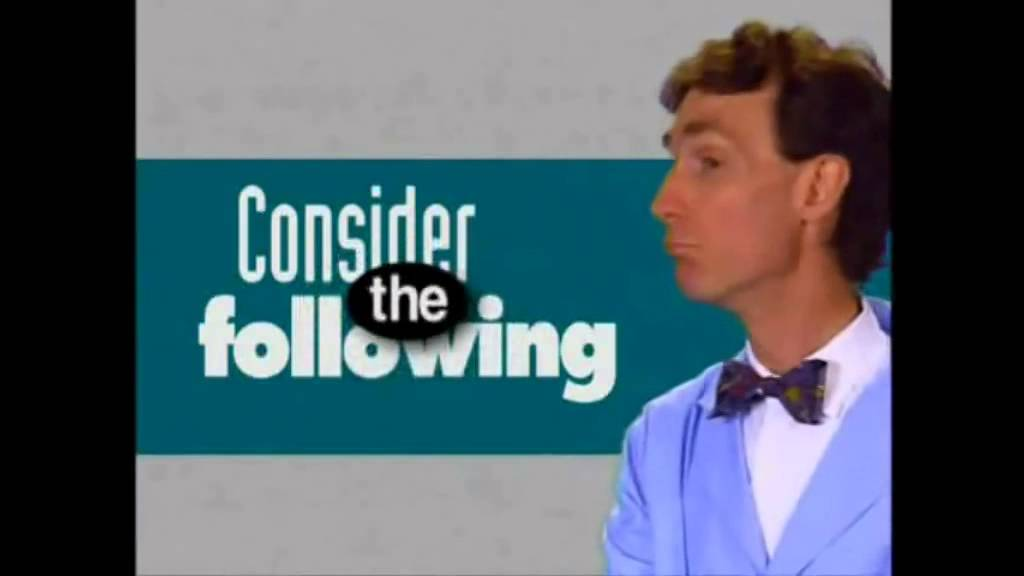
\includegraphics[width=0.7\textwidth]{../figures/consider_the_following.jpg}}
\end{center}
\end{frame}

\begin{frame}{What Do Forces Do?}
\begin{center}
   Attach a rubber band to a block and stretch the rubber band (to a fixed amount) to pull the block across a frictinless surface. We know that the block with change it's motion (accelerate).
   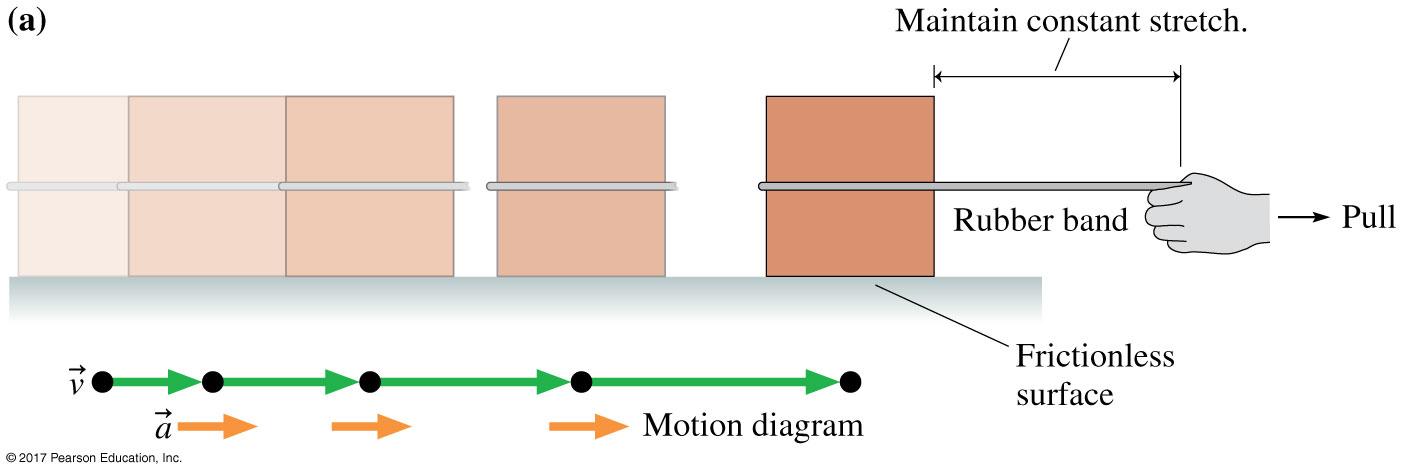
\includegraphics[width=0.5\textwidth]{../figures/05_15_FigureA.jpg}
\end{center}
\begin{itemize}
   \item<2-> What happens to the acceleration if I add a second rubber band? Does it go up/down? By how much? The forces add so you get $F'=2F$.
   \item<3-> $a$ also doubles. It turns out that the acceleration is proportional to the force applied.
\end{itemize}
   \uncover<3>{\begin{equation*}
      a \propto F \text{~~~or~~~} a = cF
   \end{equation*}
   \begin{center}
   What does {\bf proportional} mean? \\
   \uncover<4>{but what is $c$?}
   \end{center}}
\end{frame}

\begin{frame}{What Do Forces Do?}
\begin{itemize}
   \item What if I were to double the mass of the block (say from 1kg to 2kg), what would happen to the acceleration? Think of pushing a broken down car vs a broken down semi $\ldots$
   \item<2-> It's harder to change the motion of an object with large mass. In fact it turns out that the acceleration is {\bf inversely proportional} to the mass of the object.
   \begin{equation*}
      a=\frac{F}{m}
   \end{equation*}
   \begin{center}
      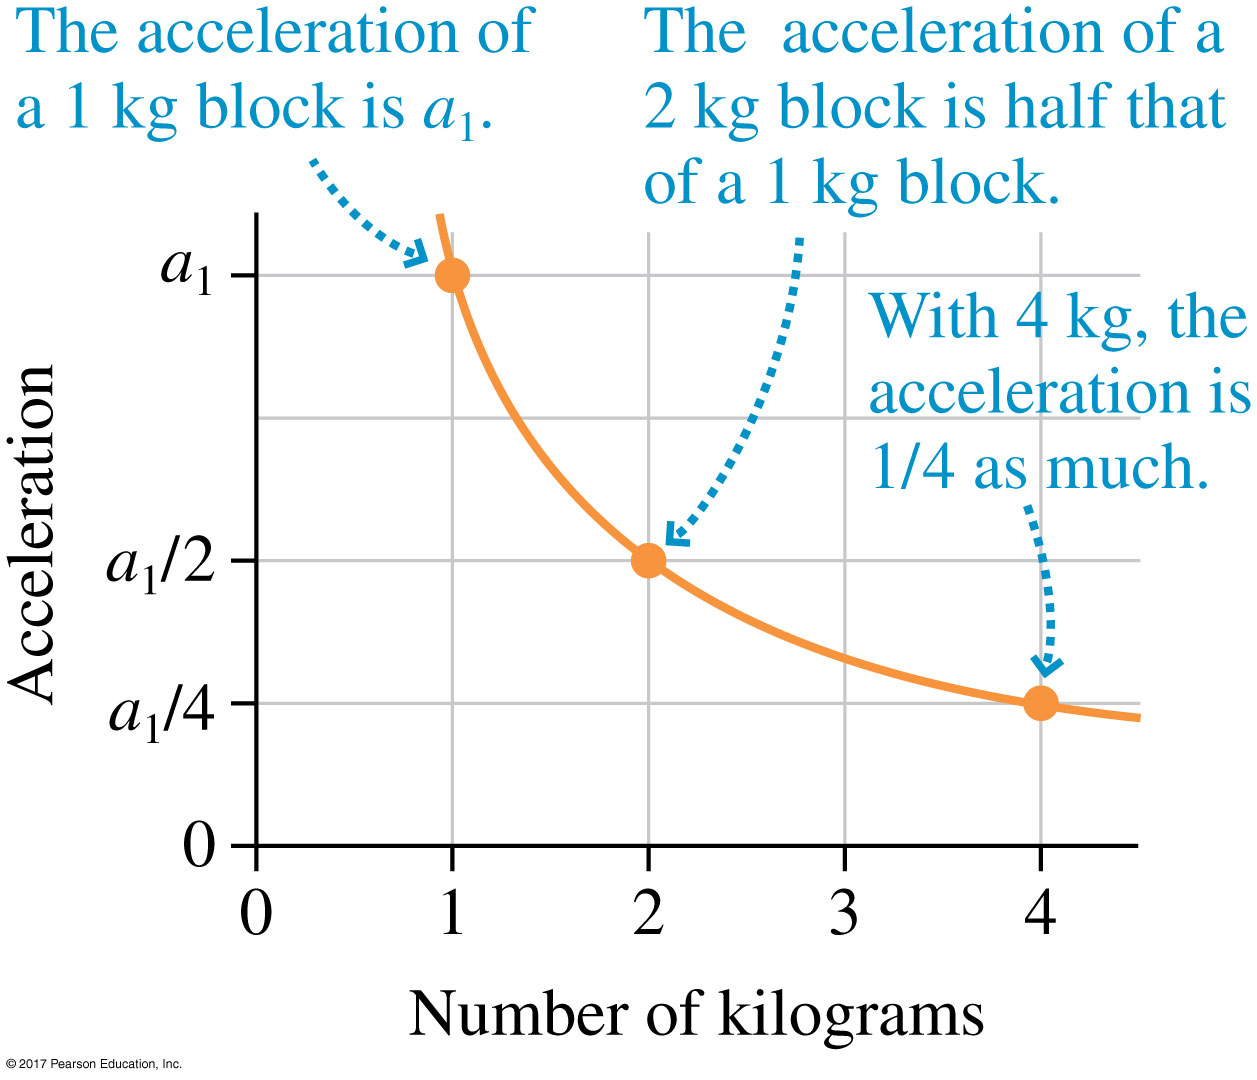
\includegraphics[width=0.4\textwidth]{../figures/05_16_Figure.jpg}
   \end{center}
\end{itemize}
\end{frame}

\begin{frame}{Quick Check}
\begin{center}
   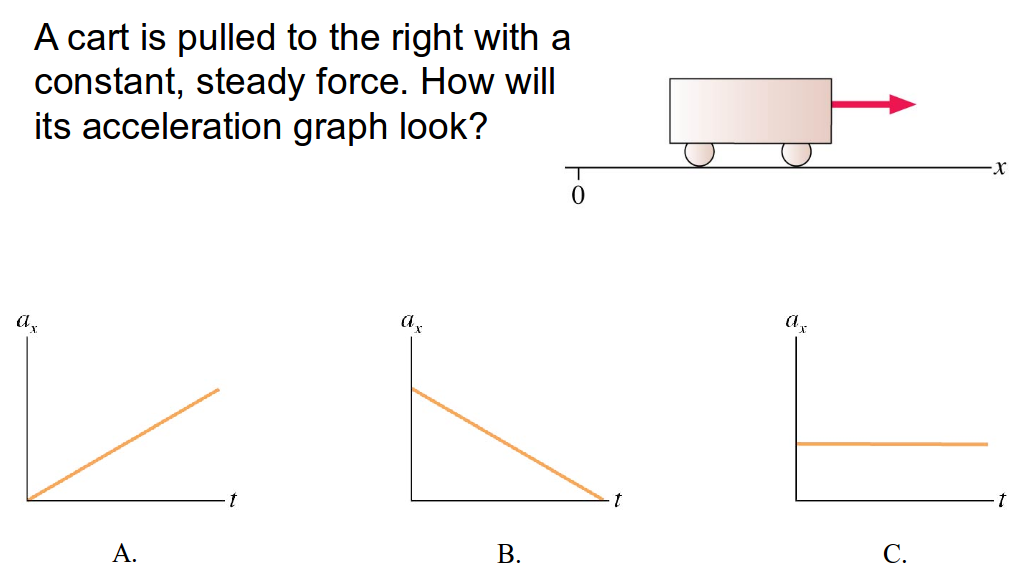
\includegraphics[width=\textwidth]{../figures/QC5_6.png}
\end{center}
\only<2>{\checkL{10.3cm}{7.4cm}}
\end{frame}

\begin{frame}{Newton - units}
\begin{itemize}
   \item Alright, so if $a=F/m \rightarrow F=ma$ then what are the units of force?
   \uncover<2>{\begin{center}
      Force Unit = kg $\times$ $\frac{\text{m}}{\text{s}^2}$ = $\frac{\text{kg m}}{\text{s}^2}$ = N
   \end{center}}
   \item<2-> This is called a {\bf newton}, so 1 N = 1 kg m/s$^2$.
\end{itemize}
\end{frame}

\begin{frame}{Inertial Mass}
\begin{itemize}
   \item 1 kg of mass is defined by a particular metal block in a vault in Paris (90\% Platinum 10\% Iridium). So it seems we could say that the mass of an object is related to how much stuff/matter it is made of.
   \item<2-> However, now we have another way (more precise way) to define the mass of an object. If the same force causes one object to accelerate twice as much as another object then it must have half as much mass.
   \item<3-> Mass {\it resists} acceleration due to a force, this is called {\bf inertia} and so we call this mass {\bf inertial mass}.
\end{itemize}
\end{frame}

\begin{frame}{Newton's 2nd Law}
\begin{itemize}
   \item When there are multiple forces acting on an object the amount and direction of the acceleration is dictated by the net force.
   \begin{equation*}
      \vec{a} = \frac{\vec{F}_{net}}{m}
   \end{equation*}
   more commonly seen as
   \begin{equation*}
      \vec{F}_{net} = m\vec{a}
   \end{equation*}
\end{itemize}
\begin{columns}
\begin{column}{0.5\textwidth}
\begin{center}
   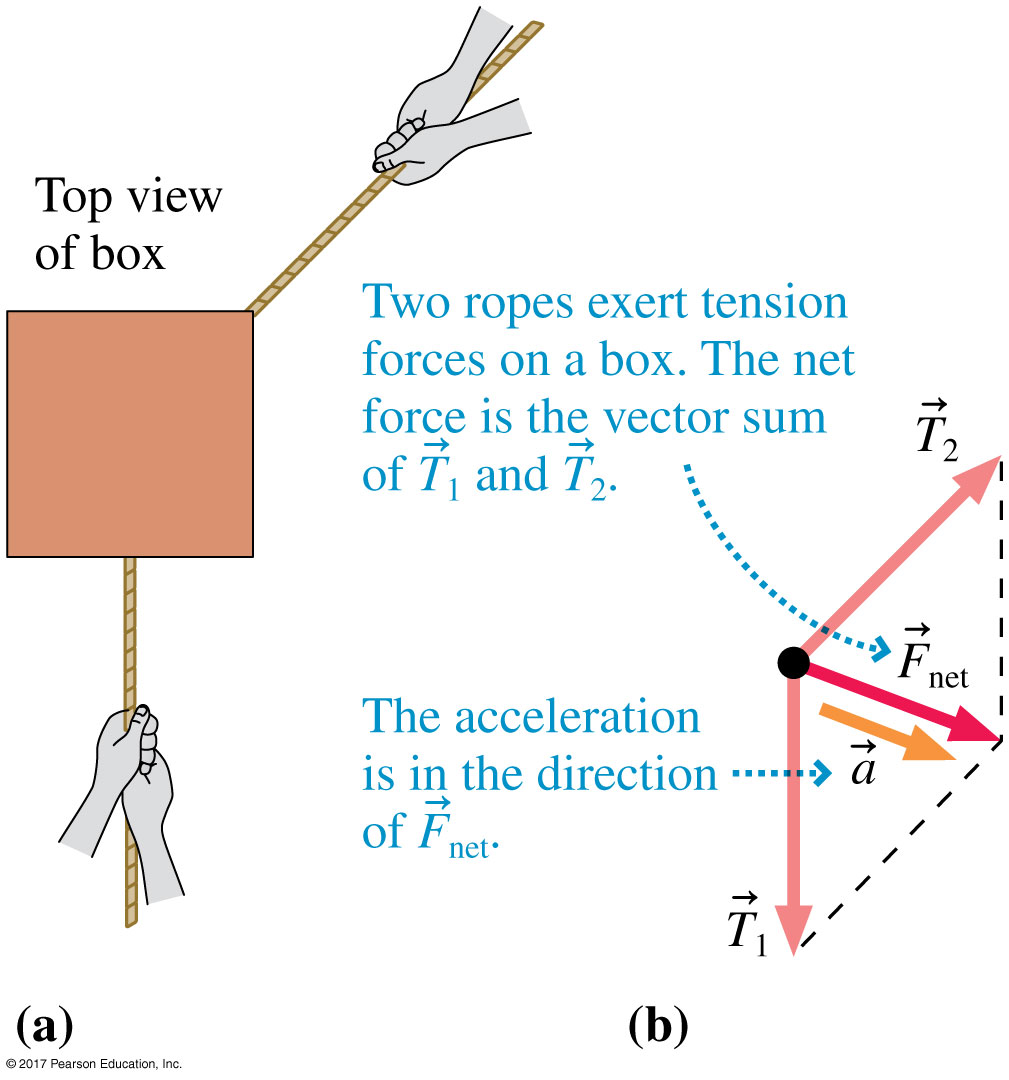
\includegraphics[width=0.90\textwidth]{../figures/05_17_Figure.jpg}
\end{center}
\end{column}
\begin{column}{0.5\textwidth}
The acceleration is {\bf NOT} $(T_1+T_2)/m$ but
\begin{equation*}
   \vec{a} = \frac{\vec{T}_1+\vec{T}_2}{m}
\end{equation*}
\end{column}
\end{columns}
\end{frame}

\begin{frame}{Newton's Laws}
\begin{itemize}
   \item Forces don't {\it overcome} eachother, they simply add together to create a net force. Forces don't compete.
   \item One more interesting aspect of forces is that when an agent exerts a force on an object, the object exerts a force on agent as well. This is called {\bf Newton's third law} and we'll talk more about it later. Think of hitting a solid brick wall \ldots your hand exerted the force, but clearly the wall exerted one back.
\end{itemize}
\end{frame}

\begin{frame}{Quick Check}
\begin{center}
   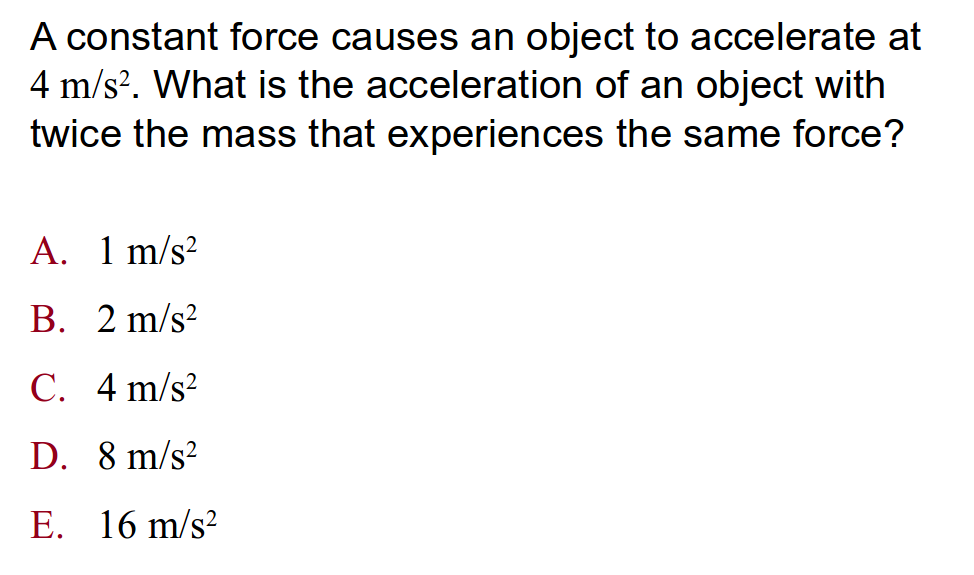
\includegraphics[width=\textwidth]{../figures/QC5_7.png}
\end{center}
\only<2>{\checkL{0.9cm}{4.8cm}}
\end{frame}

\begin{frame}{Newton's 1st Law}
\begin{itemize}
   \item An object in motion tends to \ldots \uncover<2>{stay in motion}.
   \item<3-> This is also called the law of inertia and is fully stated as 
\end{itemize}
   \uncover<3>{\begin{center}
      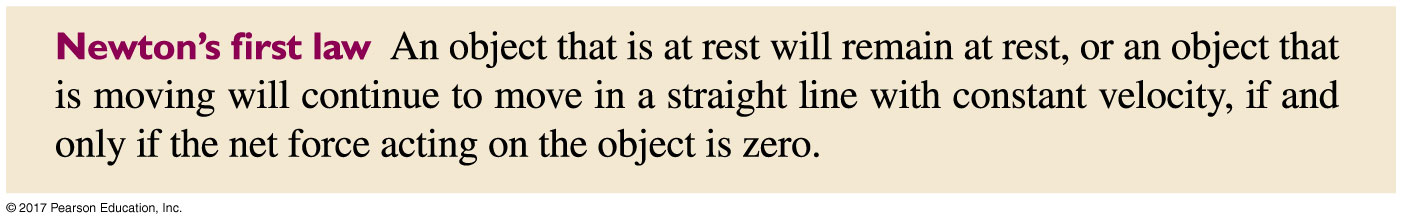
\includegraphics[width=\textwidth]{../figures/05_KeyLaw_01.jpg}
   \end{center}}
\end{frame}

\begin{frame}{Newton's 1st Law}
\begin{columns}
\begin{column}{0.5\textwidth}
\begin{itemize}
   \item An object on which the net force is zero and thus is either at rest or moving in a straight line with constant velocity is said to be in mechanical equilibrium and thus has zero acceleration.
\end{itemize}
\end{column}
\begin{column}{0.5\textwidth}
\begin{center}
   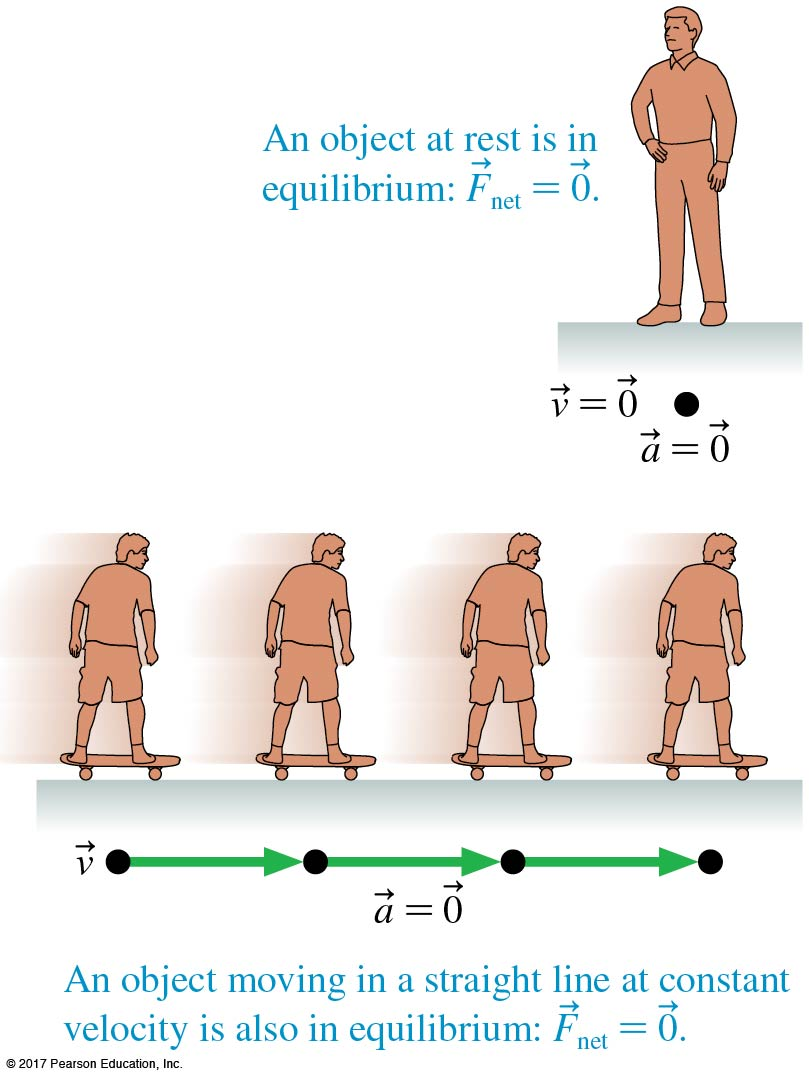
\includegraphics[width=\textwidth]{../figures/05_18_Figure.jpg}
\end{center}
\end{column}
\end{columns}
\end{frame}

\begin{frame}{Quick Check}
\begin{center}
   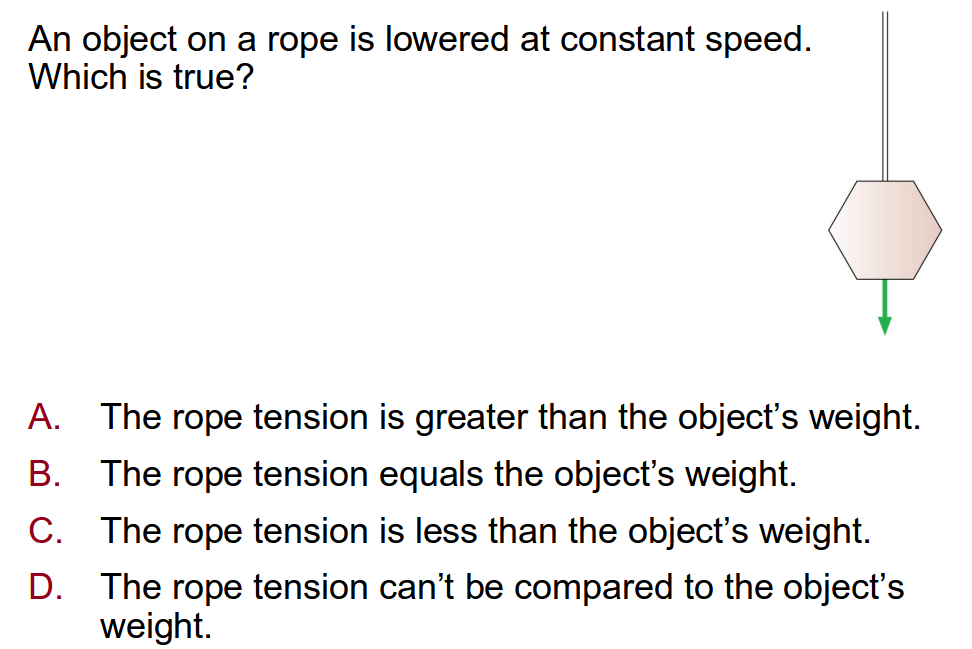
\includegraphics[width=\textwidth]{../figures/QC5_8.png}
\end{center}
\only<2>{\checkL{0.9cm}{6.2cm}}
\end{frame}

\begin{frame}{Quick Check}
\begin{center}
   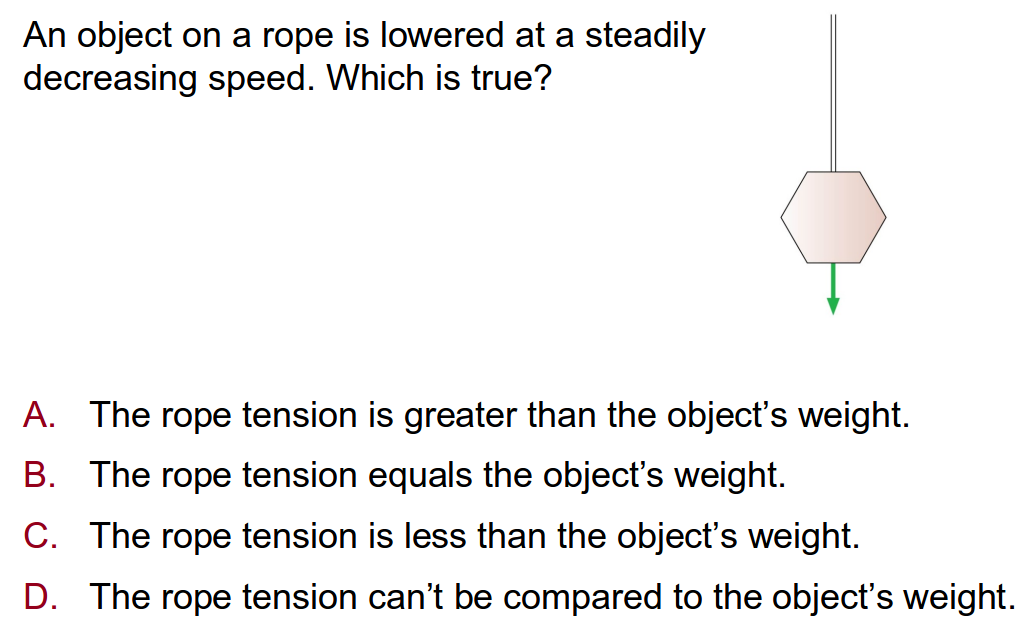
\includegraphics[width=\textwidth]{../figures/QC5_9.png}
\end{center}
\only<2>{\checkL{0.9cm}{5.5cm}}
\end{frame}

\begin{frame}{Inertial Reference Frames}
\begin{center}
   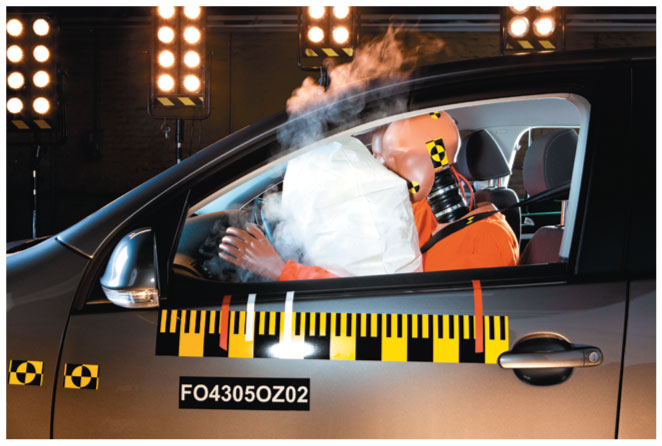
\includegraphics[width=0.5\textwidth]{../figures/05_Pg122_UnFigure.jpg}
\end{center}
\begin{itemize}
   \item Is there a force that throws this dummy into the windshield?
   \item<2-> No, it just seems like it. What is the acceleration of the dummy relative to the car?
   \begin{itemize}
      \item<3-> Large and positive
   \end{itemize}
   \item<4-> What is the acceleration of the dummy relative to the earth?
   \begin{itemize}
      \item<5-> Zero
   \end{itemize}
\end{itemize}
\end{frame}

\begin{frame}{Inertial Reference Frames}
\begin{columns}
\begin{column}{0.5\textwidth}
\begin{itemize}
   \item An {\bf inertial reference frame} is a reference frame in which Newton's laws are valid \ldots unlike the ``car" reference frame in the dummy in the car situation.
   \item Inertial reference frames are non-accelerating reference frames.
\end{itemize}
\end{column}
\begin{column}{0.5\textwidth}
\begin{center}
   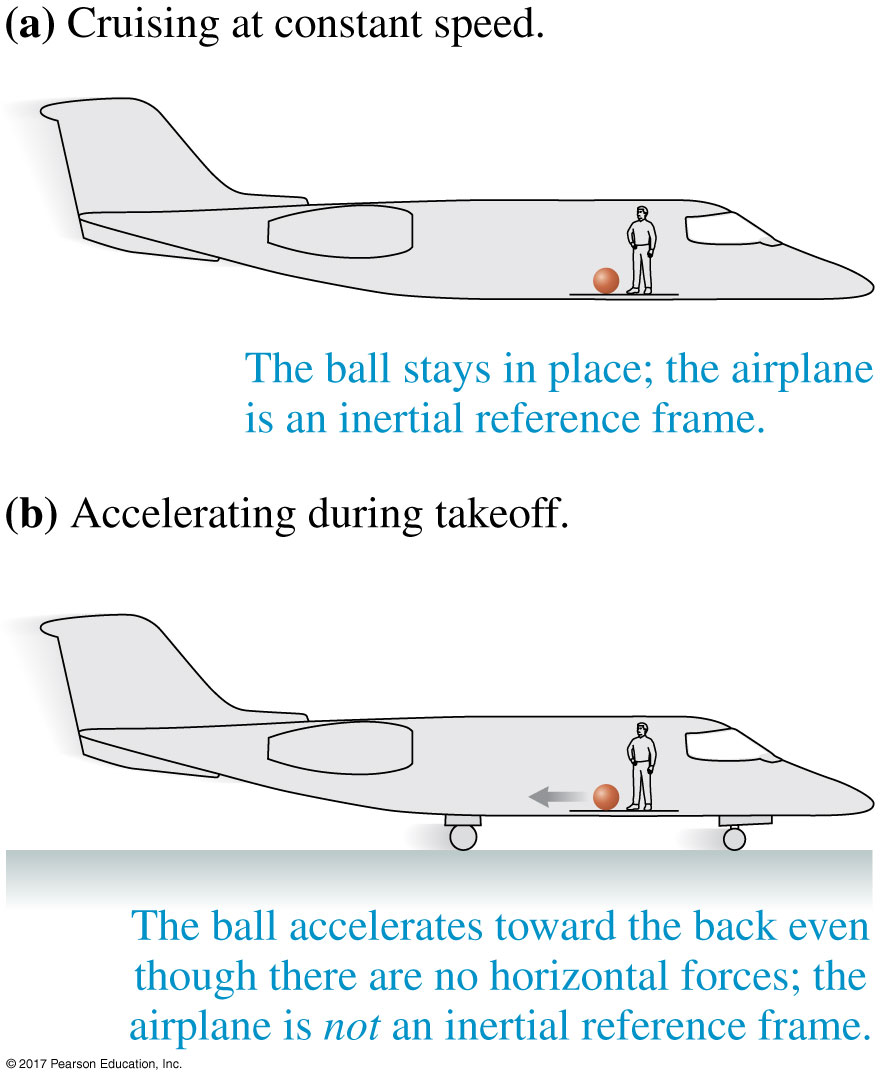
\includegraphics[width=\textwidth]{../figures/05_19_Figure.jpg}
\end{center}
\end{column}
\end{columns}
\end{frame}

\begin{frame}{Forces}
\begin{itemize}
   \item Every force has an agent which causes the force.
   \item Forces exist at the point of contact between the agent and the object (except for the few special cases of long-range forces).
   \item Forces exist due to interactions happening now, not due to what happened in the past.
   \item Consider a flying arrow.
   \begin{itemize}
      \item A pushing force was required to accelerate the arrow as it was shot.
      \item However, no force is needed to keep the arrow moving forward as it flies.
      \item It continues to move because of inertia.
   \end{itemize}
\end{itemize}
\begin{center}
   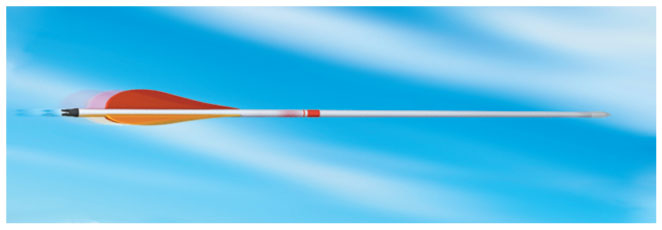
\includegraphics[width=0.5\textwidth]{../figures/05_Pg123_UnFigure.jpg}
\end{center}
\end{frame}

\begin{frame}{Quick Check}
\begin{center}
   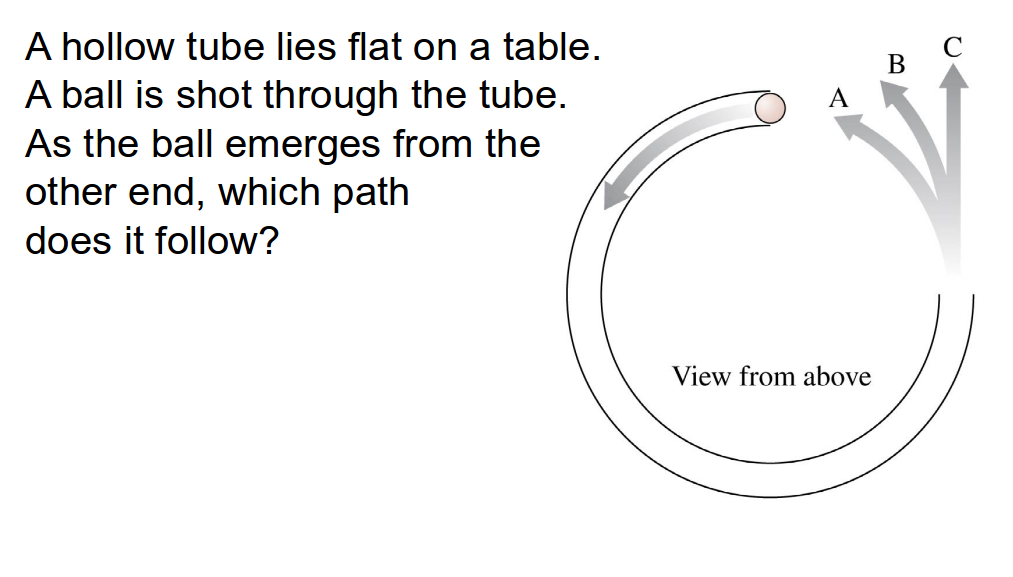
\includegraphics[width=\textwidth]{../figures/QC5_10.png}
\end{center}
\only<2>{\checkL{11.2cm}{2.0cm}}
\end{frame}

\begin{frame}{Free-Body Diagrams}
\begin{center}
   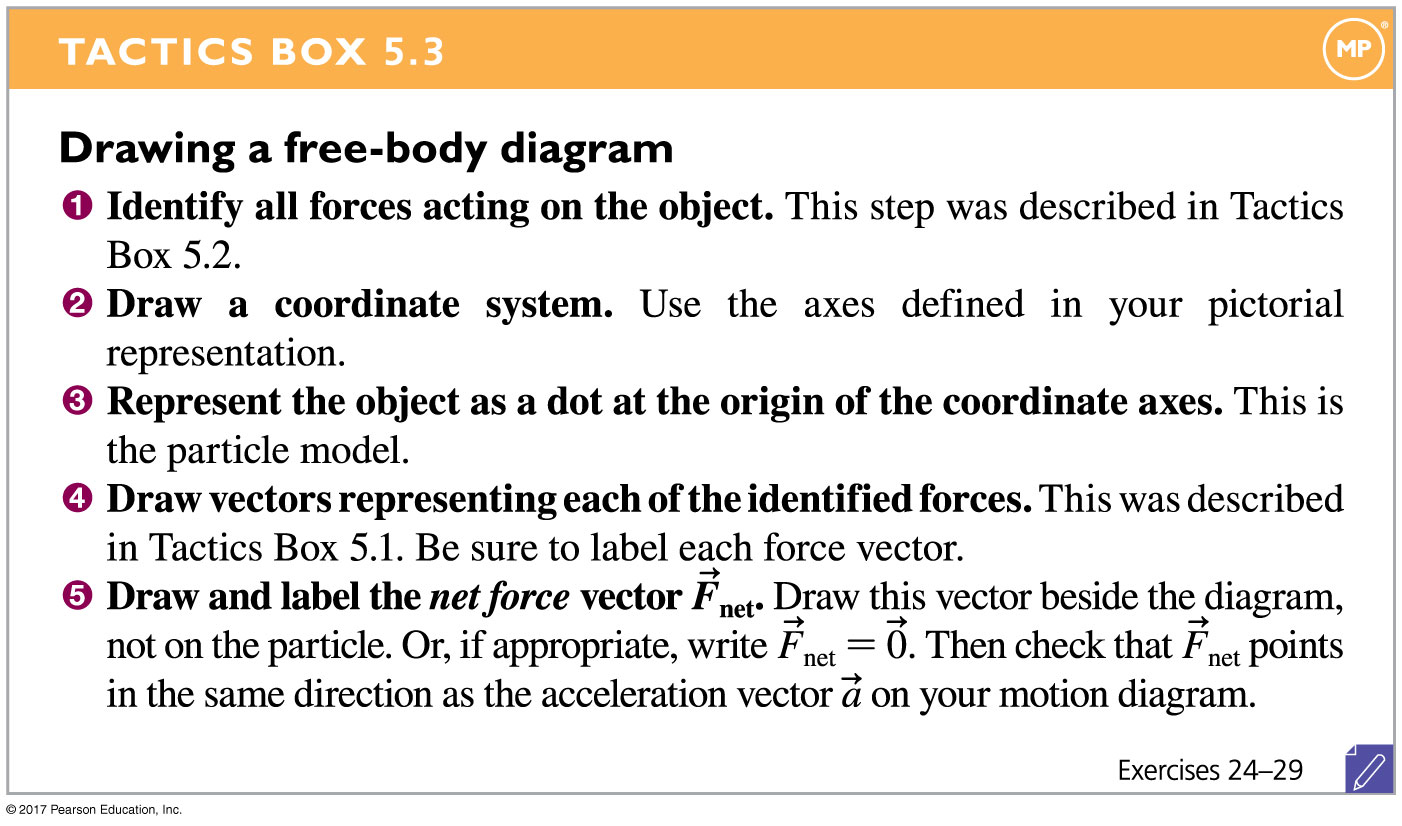
\includegraphics[width=\textwidth]{../figures/05_TacticsBox_03.jpg}
\end{center}
\end{frame}

\begin{frame}{Quick Check}
\begin{center}
   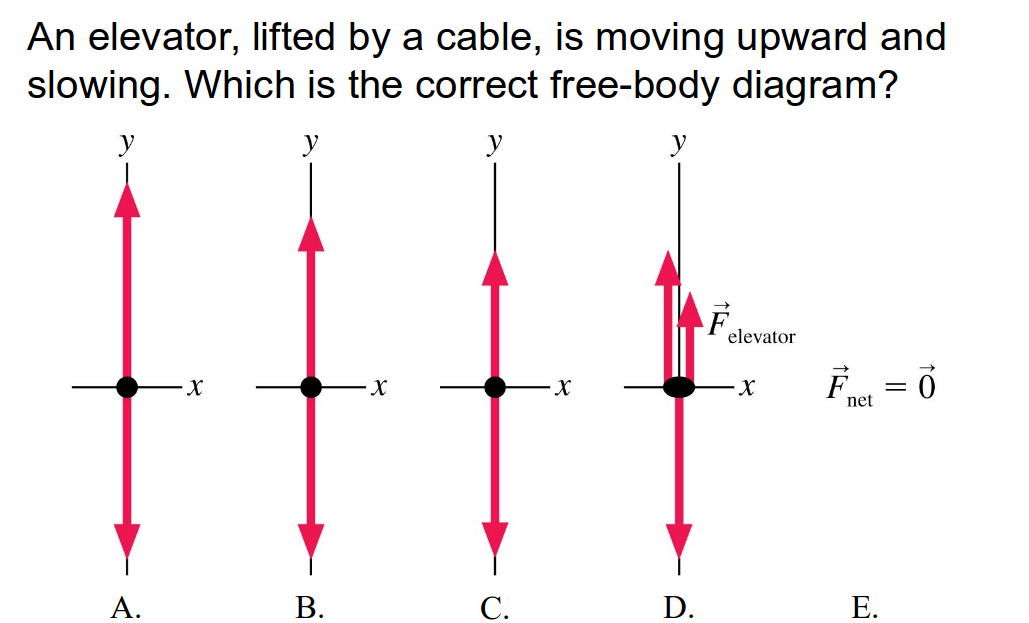
\includegraphics[width=\textwidth]{../figures/QC5_11.png}
\end{center}
\only<2>{\checkL{6.0cm}{7.8cm}}
\end{frame}

\begin{frame}{Quick Check}
\begin{center}
   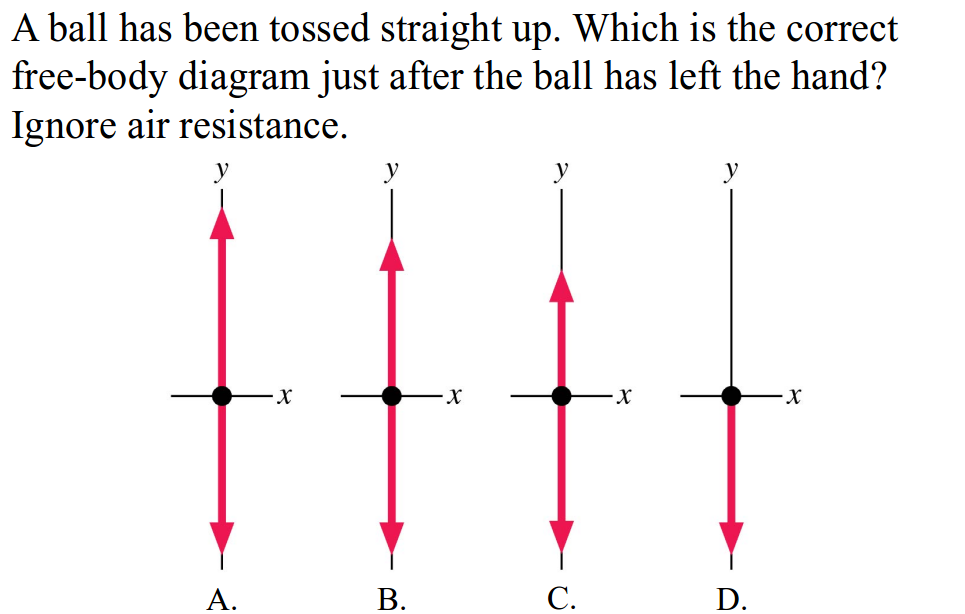
\includegraphics[width=\textwidth]{../figures/QC5_12.png}
\end{center}
\only<2>{\checkL{9.0cm}{8.2cm}}
\end{frame}

\begin{frame}{Quick Check}
\begin{center}
   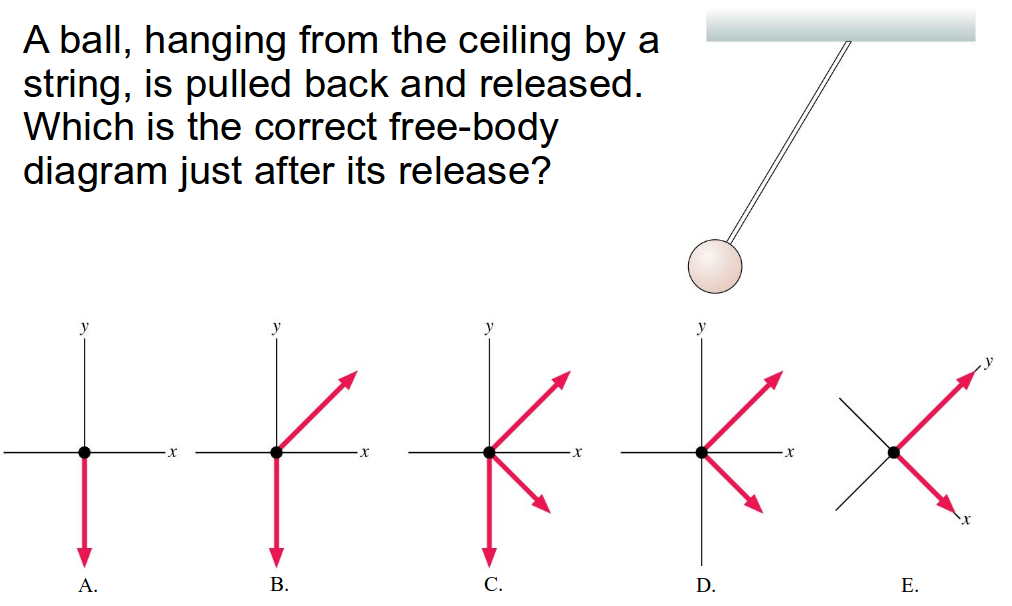
\includegraphics[width=\textwidth]{../figures/QC5_13.png}
\end{center}
\only<2>{\checkL{4.0cm}{7.7cm}}
\end{frame}

\begin{frame}{Picture References}
\tiny
Consider the Following (accessed 25 Sep 2017) \href{https://i.ytimg.com/vi/71VT6oTto1g/maxresdefault.jpg}{https://i.ytimg.com/vi/71VT6oTto1g/maxresdefault.jpg} \\
\end{frame}

\end{document}
